\documentclass{standalone}
% packages
\usepackage{tikz}
\usepackage{tikz-qtree}
\usetikzlibrary{positioning,arrows.meta,quotes,calc}
% tikz setup
\tikzset{%
  arrow/.style    = { ->, >=Latex,  very thick, rounded corners, fill = #1, draw = #1 },
  tbox/.style     = { fill = #1!20!white, draw = #1!80!white, thick, align = center, rounded corners,
    minimum width = 0.8cm, minimum height = 0.6cm, node distance = 1.5cm },
}
% colors
\newcommand{\colorx}{blue}
\newcommand{\colori}{\colorx!40!white}
\newcommand{\coloro}{\colorx!40!black}
\newcommand{\colort}{\colorx!50!green}
\newcommand{\colord}{\colorx!50!red}
% global turn labels on/off
\newcommand{\arrowlabel}[1]{{}}
\newcommand{\nodelabel}[1]{{#1}}
% document
\begin{document}
  % ================================================================================================
  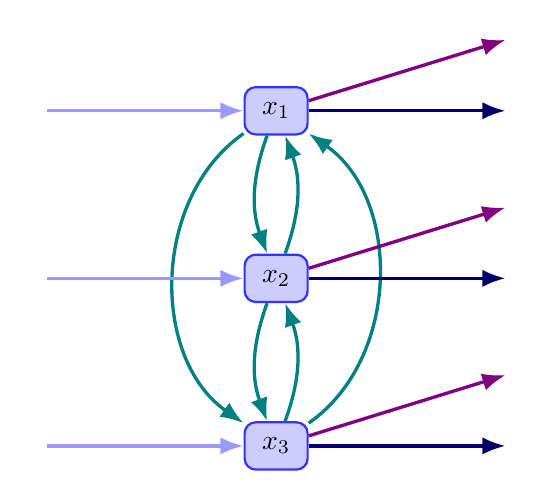
\begin{tikzpicture}
    % nodes ----------------------------------------------------------------------------------------
    % main 3 nodes
    \node(x1) [tbox=\colorx] at (0.0,0.0)       {\nodelabel{$x_1$}};
    \node(x2) [tbox=\colorx, below = of x1]     {\nodelabel{$x_2$}};
    \node(x3) [tbox=\colorx, below = of x2]     {\nodelabel{$x_3$}};
    % input nodes (no tbox)
    \node(i1) [, left  = 2.5cm of x1] {};%{\nodelabel{$e_1$}};
    \node(i2) [, left  = 2.5cm of x2] {};%{\nodelabel{$e_2$}};
    \node(i3) [, left  = 2.5cm of x3] {};%{\nodelabel{$e_3$}};
    % output nodes (no tbox)
    \node(o1) [,   right = 2.5cm of x1] {}; %{\nodelabel{$o_3$}};
    \node(o2) [,   right = 2.5cm of x2] {}; %{\nodelabel{$o_3$}};
    \node(o3) [,   right = 2.5cm of x3] {}; %{\nodelabel{$o_3$}};
    % mortality nodes (no tbox)
    \node(d1) [,   above right = 0.5cm and 2.5cm of x1] {};
    \node(d2) [,   above right = 0.5cm and 2.5cm of x2] {};
    \node(d3) [,   above right = 0.5cm and 2.5cm of x3] {};
    % arrows ---------------------------------------------------------------------------------------
    % turnover
    \draw[arrow=\colort] (x1) edge["\arrowlabel{$\zeta_{12}$}", swap, bend right=20] (x2); 
    \draw[arrow=\colort] (x2) edge["\arrowlabel{$\zeta_{21}$}", swap, bend right=20] (x1);
    \draw[arrow=\colort] (x3) edge["\arrowlabel{$\zeta_{32}$}", swap, bend right=20] (x2); 
    \draw[arrow=\colort] (x2) edge["\arrowlabel{$\zeta_{23}$}", swap, bend right=20] (x3);
    \draw[arrow=\colort] (x1) edge["\arrowlabel{$\zeta_{13}$}", swap, bend right=55, near end] (x3); 
    \draw[arrow=\colort] (x3) edge["\arrowlabel{$\zeta_{31}$}", swap, bend right=55, near end] (x1);
    % entry
    \draw[arrow=\colori] (i1) edge["\arrowlabel{$\nu$}", near start] (x1);
    \draw[arrow=\colori] (i2) edge["\arrowlabel{$\nu$}", near start] (x2);
    \draw[arrow=\colori] (i3) edge["\arrowlabel{$\nu$}", near start] (x3);
    % exit
    \draw[arrow=\coloro] (x1) edge["\arrowlabel{$\mu$}", near end]   (o1);
    \draw[arrow=\coloro] (x2) edge["\arrowlabel{$\mu$}", near end]   (o2);
    \draw[arrow=\coloro] (x3) edge["\arrowlabel{$\mu$}", near end]   (o3);
    % mortality arrows
    \draw[arrow=\colord] (x1) edge["\arrowlabel{$\phi_1$}", near end]  (d1);
    \draw[arrow=\colord] (x2) edge["\arrowlabel{$\phi_2$}", near end]  (d2);
    \draw[arrow=\colord] (x3) edge["\arrowlabel{$\phi_3$}", near end]  (d3);
  \end{tikzpicture}
  % ================================================================================================
\end{document}
% eof
